\section{Derivatives and Rates of Change} \label{S:2.1.DerivativePt}

\begin{goals}
\item How is the average rate of change of a function on a given interval defined, and what does this quantity measure?
\item How is the instantaneous rate of change of a function at a particular point defined?  How is the instantaneous rate of change linked to average rate of change?
\item What is the derivative of a function at a given point?  What does this derivative value measure? How do we interpret the derivative value graphically?
\item How are limits used formally in the computation of derivatives? 
\item In contexts other than the position of a moving object, what does the derivative of a function measure?
\item What are the units on the derivative function $f'$, and how are they related to the units of the original function $f$?
\item What is a central difference, and how can one be used to estimate the value of the derivative at a point from given function data?
\item Given the value of the derivative of a function at a point, what can we infer about how the value of the function changes nearby?
\end{goals}

%--------------------------------------
% SUBSECTION INTRODUCTION
%--------------------------------------
\subsection*{Introduction}

An idea that sits at the foundations of calculus is the \emph{instantaneous rate of change} of a function.  This rate of change is always considered with respect to change in the input variable, often at a particular fixed input value.  This is a generalization of the notion of instantaneous velocity and essentially allows us to consider the question "how do we measure how fast a particular function is changing at a given point?"  When the original function represents the position of a moving object, this instantaneous rate of change is precisely velocity, and might be measured in units such as feet per second.  But in other contexts, instantaneous rate of change could measure the number of cells added to a bacteria culture per day, the number of additional gallons of gasoline consumed by going one mile per additional mile per hour in a car's velocity, or the number of dollars added to a mortgage payment for each percentage increase in interest rate.  Regardless of the presence of a physical or practical interpretation of a function, the instantaneous rate of change may also be interpreted geometrically in connection to the function's graph, and this connection is also foundational to many of the main ideas in calculus.

In what follows, we will introduce terminology and notation that makes it easier to talk about the instantaneous rate of change of a function at a point.  In addition, just as instantaneous velocity is defined in terms of average velocity, the more general instantaneous rate of change will be connected to the more general average rate of change.  Recall that for a moving object with position function $s$, its average velocity on the time interval $t = a$ to $t = a+h$ is given by the quotient 
\[ AV_{[a,a+h]} = \frac{s(a+h)-s(a)}{h}. \]
In a similar way, we make the following definition for an arbitrary function $y = f(x).$

\definition{Average Rate of Change}{ %DEFINITION
For a function $f$, the \emph{average rate of change}\index{average rate of change} of $f$ on the interval $[a,a+h]$ is given by the value
\[ AV_{[a,a+h]} = \frac{f(a+h)-f(a)}{h}. \]
} % end definition

Equivalently, if we want to consider the average rate of change of $f$ on $[a,b]$, we compute 
\[ AV_{[a,b]} = \frac{f(b)-f(a)}{b-a}. \]
It is essential to understand how the average rate of change of $f$ on an interval is connected to its graph.

%\newpage % The figure in the preview activity bleeds onto the previous page.  If it gets `worked out', delete this line.

\begin{marginfigure}
\includegraphics{figures/1_3_PA1.eps}
\caption{Plot of $y = f(x)$ for Preview Activity~\ref{PA:2.1}.} \label{fig:2.1.PA1}
\end{marginfigure}

\begin{pa} \label{PA:2.1}
Suppose that $f$ is the function given by the graph in Figure~\ref{fig:2.1.PA1} and that $a$ and $a+h$ are the input values as labeled on the $x$-axis.  Use the graph in Figure~\ref{fig:2.1.PA1} to answer the following questions.

\ba
	\item Locate and label the points $(a,f(a))$ and $(a+h, f(a+h))$ on the graph.
	\item Construct a right triangle whose hypotenuse is the line segment from $(a,f(a))$ to $(a+h,f(a+h))$.  What are the lengths of the respective legs of this triangle?
	\item What is the slope of the line that connects the points $(a,f(a))$ and $(a+h, f(a+h))$?
	\item Write a meaningful sentence that explains how the average rate of change of the function on a given interval and the slope of a related line are connected.
\ea
\end{pa} \afterpa % PREVIEW ACTIVITY 

%-------------------------------------------------
% SUBSECTION DERIVATIVE AT A POINT
%-------------------------------------------------
\subsection*{The Derivative of a Function at a Point}

Just as we defined instantaneous velocity in terms of average velocity, we now define the instantaneous rate of change of a function at a point in terms of the average rate of change of the function $f$ over related intervals.  In addition, we give a special name to "the instantaneous rate of change of $f$ at $a$,"\index{instantaneous rate of change} calling this quantity "the \emph{derivative} of $f$ at $a$," with this value being represented by the shorthand notation $f'(a)$.   Specifically, we make the following definition.

\definition{Derivative at a Point}{ %DEFINITION
Let $f$ be a function and $x = a$ a value in the function's domain.  We define the \emph{derivative of $f$ with respect to $x$ evaluated at $x = a$}\index{derivative!definition}, denoted $f'(a)$, by the formula
\[ f'(a) = \lim_{h \to 0} \frac{f(a+h)-f(a)}{h}, \]
provided this limit exists. We say that a function that has a derivative at $x = a$ is \emph{differentiable}\index{differentiable} at $x = a$.
} % end definition

Aloud, we read the symbol $f'(a)$ as either "$f$-prime at $a$" or "the derivative of $f$ evaluated at $x = a$."  Much of the next several chapters will be devoted to understanding, computing, applying, and interpreting derivatives.  For now, we make the following important notes.
\begin{itemize}
	\item The derivative of $f$ at the value $x = a$ is defined as the limit of the average rate of change of $f$ on the interval $[a,a+h]$ as $h \to 0$.  It is possible for this limit not to exist, so not every function has a derivative at every point.
	\item The derivative is a generalization of the instantaneous velocity of a position function:  when $y = s(t)$ is a position function of a moving body, $s'(a)$ tells us the instantaneous velocity of the body at time $t=a$.
	\item Because the units on $\frac{f(a+h)-f(a)}{h}$ are ``units of $f$ per unit of $x$,'' the derivative has these very same units.  For instance, if $s$ measures position in feet and $t$ measures time in seconds, the units on $s'(a)$ are feet per second. 
	\item Because the quantity $\frac{f(a+h)-f(a)}{h}$ represents the slope of the line through $(a,f(a))$ and $(a+h, f(a+h))$, when we compute the derivative we are taking the limit of a collection of slopes of lines, and thus the derivative itself represents the slope of a particularly important line.
\end{itemize}
While all of the above ideas are important and we will add depth and perspective to them through additional time and study, for now it is most essential to recognize how the derivative of a function at a given value represents the slope of a certain line.  Thus, we expand upon the last bullet item above.

As we move from an average rate of change to an instantaneous one, we can think of one point as "sliding towards" another.  In particular, provided the function has a derivative at $(a,f(a))$, the point $(a+h,f(a+h))$ will approach $(a,f(a))$ as $h \to 0$.  Because this process of taking a limit is a dynamic one, it can be helpful to use computing technology to visualize what the limit is accomplishing.  While there are many different options\sidenote[][-1in]{For a helpful collection of java applets, consider the work of David Austin of Grand Valley State University at \href{http://gvsu.edu/s/5r}{\texttt{http://gvsu.edu/s/5r}}, and the particularly relevant example at \href{http://gvsu.edu/s/5s}{\texttt{http://gvsu.edu/s/5s}}.  For applets that have been built in Geogebra, a nice example is the work of Marc Renault of Shippensburg University at \href{http://gvsu.edu/s/5p}{\texttt{http://gvsu.edu/s/5p}}, with the example at \href{http://gvsu.edu/s/5q}{\texttt{http://gvsu.edu/s/5q}} being especially fitting for our work in this section.  There are scores of other examples posted by other authors on the internet.}, one of the best is a java applet in which the user is able to control the point that is moving.   See the examples referenced in the footnote here, or consider building your own, perhaps using the fantastic free program Geogebra\sidenote{Available for free download from \href{http://geogebra.org}{\texttt{http://geogebra.org}}.}.

\begin{figure*} % MARGIN FIGURE
\begin{center}
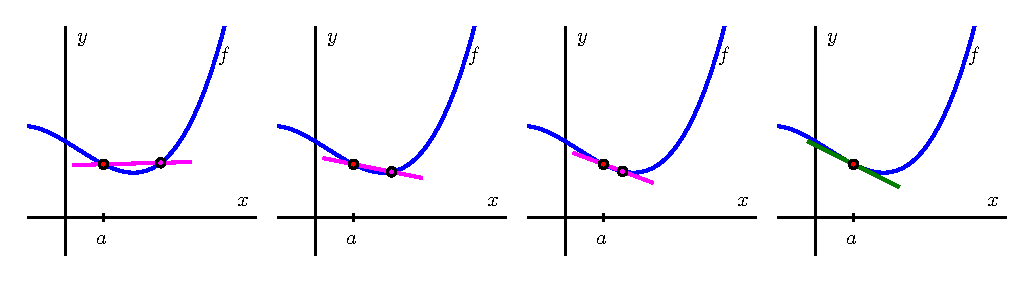
\includegraphics{figures/1_3_SecToTanSeq.eps} %figure ACTIVE
\caption{A sequence of secant lines approaching the tangent line to $f$ at $(a,f(a))$.} \label{fig:2.1.SeqToTanSeq}
\end{center}
\end{figure*}

In Figure~\ref{fig:2.1.SeqToTanSeq}, we provide a sequence of figures with several different lines through the points $(a, f(a))$ and $(a+h,f(a+h))$ that are generated by different values of $h$.  These lines (shown in the first three figures in magenta), are often called \emph{secant lines} \index{secant line} to the curve $y = f(x)$.  A secant line to a curve is simply a line that passes through two points that lie on the curve.  For each such line, the slope of the secant line is $m = \frac{f(a+h) - f(a)}{h}$, where the value of $h$ depends on the location of the point we choose.  We can see in the diagram how, as $h \to 0$, the secant lines start to approach a single line that passes through the point $(a,f(a))$.  In the situation where the limit of the slopes of the secant lines exists, we say that the resulting value is the slope of the \emph{tangent line} to the curve.  This tangent line\index{tangent line} (shown in the right-most figure in green) to the graph of $y = f(x)$ at the point $(a,f(a))$ is the line through $(a,f(a))$ whose slope is $m = f'(a)$.  

\begin{marginfigure} % MARGIN FIGURE
\margingraphics{figures/1_3_SecToTan.eps} %FIGURE ACTIVE 
\caption{A sequence of secant lines approaching the tangent line to $f$ at $(a,f(a))$.  At right, we zoom in on the point $(a,f(a))$.  The slope of the tangent line (in green) to $f$ at $(a,f(a))$ is given by $f'(a)$.} \label{fig:2.1.SeqToTan}
\end{marginfigure}

As we will see in subsequent study, the existence of the tangent line at $x = a$ is connected to whether or not the function $f$ looks like a straight line when viewed up close at $(a,f(a))$, which can also be seen in Figure~\ref{fig:2.1.SeqToTan}, where we combine the four graphs in Figure~\ref{fig:2.1.SeqToTanSeq} into the single one on the left, and then we zoom in on the box centered at $(a,f(a))$, with that view expanded on the right (with two of the secant lines omitted).  Note how the tangent line sits relative to the curve $y = f(x)$ at $(a,f(a))$ and how closely it resembles the curve near $x = a$.

At this time, it is most important to note that $f'(a)$, the instantaneous rate of change of $f$ with respect to $x$ at $x = a$, also measures the slope of the tangent line\index{tangent line!slope} to the curve $y = f(x)$ at $(a,f(a))$.  The following example demonstrates several key ideas involving the derivative of a function.

\begin{example} \label{Ex:2.1.Eg1}
For the function given by $f(x) = x - x^2$, use the limit definition of the derivative to compute $f'(2)$.  In addition, discuss the meaning of this value and draw a labeled graph that supports your explanation. 

\solution From the limit definition, we know that
$$f'(2) = \lim_{h \to 0} \frac{f(2+h)-f(2)}{h}.$$
Now we use the rule for $f$, and observe that $f(2) = 2 - 2^2 = -2$ and $f(2+h) = (2+h) - (2+h)^2.$  Substituting these values into the limit definition, we have that
$$f'(2) = \lim_{h \to 0} \frac{(2+h) - (2+h)^2 -  (-2)}{h}.$$
Observe that with $h$ in the denominator and our desire to let $h \to 0$, we have to wait to take the limit (that is, we wait to actually let $h$ approach $0$).  Thus, we do additional algebra.  Expanding and distributing in the numerator,
$$f'(2) = \lim_{h \to 0} \frac{2+h - 4 - 4h - h^2 + 2}{h}.$$
Combining like terms, we have
$$f'(2) = \lim_{h \to 0} \frac{ -3h - h^2}{h}.$$
Next, we observe that there is a common factor of $h$ in both the numerator and denominator, which allows us to simplify and find that
$$f'(2) = \lim_{h \to 0} (-3-h).$$
Finally, we are able to take the limit as $h \to 0$, and thus conclude that $f'(2) = -3$.

Now, we know that $f'(2)$ represents the slope of the tangent line to the curve $y = x - x^2$ at the point $(2,-2)$; $f'(2)$ is also the instantaneous rate of change of $f$ at the point $(2,-2)$.  Graphing both the function and the line through $(2,-2)$ with slope $m = f'(2) = -3$, we indeed see that by calculating the derivative, we have found the slope of the tangent line at this point, as shown in Figure~\ref{fig:2.1.Eg1}.
\end{example}

\begin{marginfigure}[-6cm]
\margingraphics{figs/2/2-1_Eg1.pdf} %Tangent line ex 1.3 active
\caption{The tangent line to $y = x - x^2$ at the point $(2,-2)$.}\label{fig:2.1.Eg1}
\end{marginfigure} % EXAMPLE

\begin{marginfigure}[1cm]
\margingraphics{figures/figtangent1} %FIG EXAMPLE 33 apex
\caption{A graph of $f(x) = 3x^2+5x-7$ and its tangent lines at $x=1$ and $x=3$.}\label{fig:2.1.Eg3}
\end{marginfigure}

\begin{example} \label{Ex:2.1.Eg3}
Let $f(x) = 3x^2+5x-7$. Find: 
\begin{enumerate*}[1)]
\item $f'(1)$; 	
\item the equation of the tangent line to the graph of $f$ at $x=1$; 
\item $f'(3)$; and 
\item the equation of the tangent line to the graph $f$ at $x=3$.
\end{enumerate*}
	
\solution
\begin{enumerate}[1)]
\item We compute this directly using the definition of the derivative at a point.
\begin{align*}
f'(1) &= \lim_{h \to 0} \frac{f(1+h)-f(1)}{h} \\
&=	\lim_{h \to 0} \frac{3(1+h)^2+5(1+h)-7 - (3(1)^2+5(1)-7)}{h}\\
&=	\lim_{h\to 0} \frac{3h^2+11h}{h}\\
&= 	\lim_{h\to 0} 3h+11=11.
%&= 11.
\end{align*}

\item The tangent line at $x=1$ has slope $f'(1)$ and goes through the point $(1,f(1)) = (1,1)$. Thus the tangent line has equation, in point-slope form, $y = 11(x-1) + 1$. In slope-intercept form we have $y = 11x-10$.
	
\item Again, using the definition,
\begin{align*}
f'(3) &=	\lim_{h \to 0} \frac{f(3+h)-f(3)}{h} \\
&=	\lim_{h \to 0} \frac{3(3+h)^2+5(3+h)-7 - (3(3)^2+5(3)-7)}{h} \\
&=	\lim_{h \to 0} \frac{3h^2+23h}{h}\\
&= \lim_{h \to 0} 3h+23 = 23
%&= 23.
\end{align*}
	
\item The tangent line at $x=3$ has slope $23$ and goes through the point $(3,f(3)) = (3,35)$. Thus the tangent line has equation $y=23(x-3)+35 = 23x-34$.
\end{enumerate}
\end{example} % EXAMPLE APEX example 31

The following activities will help you explore a variety of key ideas related to derivatives.

\begin{activity} \label{A:2.1.1}
Consider the function $f$ whose formula is $\ds f(x) = 3 - 2x$.
\ba
	\item What familiar type of function is $f$?  What can you say about the slope of $f$ at every value of $x$?
	\item Compute the average rate of change of $f$ on the intervals $[1,4]$, $[3,7]$, and $[5,5+h]$; simplify each result as much as possible.  What do you notice about these quantities?
	\item Use the limit definition of the derivative to compute the exact instantaneous rate of change of $f$ with respect to $x$ at the value $a = 1$.  That is, compute $f'(1)$ using the limit definition.  Show your work.  Is your result surprising?
	\item Without doing any additional computations, what are the values of $f'(2)$, $f'(\pi)$, and $f'(-\sqrt{2})$?  Why?
\ea
\end{activity}
\begin{smallhint}
\ba
	\item If $f(x) = 3x^2 + 2x - 4$, we say ``$f$ is quadratic.''  If $f(x) = 5 e^{2x-1}$, we say ``$f$ is exponential.''  What do we say about $f(x) = 3-2x$.  
	\item Remember that to compute the average rate of change of $f$ on $[a,b]$, we calculate $\frac{f(b)-f(a)}{b-a}$.
	\item Observe that $f(1+h) = 3 - 2(1+h) = 3 - 2 - 2h = 1 - 2h$.
	\item Think about the how the graph of $f$ appears.  What is the same at every point?
\ea
\end{smallhint}
\begin{bighint}
\ba
	\item Observe that the function $f$ is of the form $f(x) = mx + b$.
	\item To compute the average rate of change of $f$ on $[1,4]$, we calculate $\frac{f(4)-f(1)}{4-1}$.
	\item Note that $f(1+h) - f(1) = (3 - 2(1+h)) - (3-2) = 3 - 2 - 2h - 1 = -2h$.
	\item Remember that $f'(a)$ represents the slope of the function $f$ at the value $a$.
\ea
\end{bighint}
\begin{activitySolution}
\ba
	\item Because $f(x) = 3 - 2x$ is of the form $f(x) = mx + b$, we call $f$ a \emph{linear} function.
	\item The average rate of change on $[1,4]$ is $\frac{f(4)-f(1)}{4-1} = \frac{-5 - 1}{3} = -2$.  Similar calculations show the average rate of change on $[3,7]$ is also $-2$.  On $[5,5+h]$, observe that 
	$$\frac{f(5+h)-f(5)}{h} = \frac{3-2(5+h) - (3-10)}{h} = \frac{3 - 10 - 2h + 7}{h} = \frac{-2h}{h} = -2.$$
	\item Using the limit definition of the derivative, we find that
	\begin{eqnarray*}
		f'(1) & = & \lim_{h \to 0} \frac{f(1+h) - f(1)}{h} \\
			& = & \lim_{h \to 0} \frac{(3 - 2(1+h)) - (3-2)}{h} \\
			& = & \lim_{h \to 0} \frac{3 - 2 - 2h - 1}{h} \\
			& = & \lim_{h \to 0} \frac{-2h}{h} \\
			& = & \lim_{h \to 0} -2 \\
			& = & -2.
	\end{eqnarray*}
\ea
\end{activitySolution}
\aftera % ACTIVITY

\begin{marginfigure}[9cm]	
\margingraphics{figures/1_3_Act2.eps}
\caption{Axes for plotting $y = s(t)$ in Activity~\ref{A:2.1.2}.} \label{fig:2.1.Act2}
\end{marginfigure}

\begin{activity}  \label{A:2.1.2}
A water balloon is tossed vertically in the air from a window.  The balloon's height in feet at time $t$ in seconds after being launched is given by $s(t) = -16t^2 + 16t + 32$. Use this function to respond to each of the following questions.
\ba
	\item Sketch an accurate, labeled graph of $s$ on the axes provided in Figure~\ref{fig:2.1.Act2}.  You should be able to do this without using computing technology.
		
	\item Compute the average rate of change of $s$ on the time interval $[1,2]$.  Include units on your answer and write one sentence to explain the meaning of the value you found.  
	\item Use the limit definition to compute the instantaneous rate of change of $s$ with respect to time, $t$, at the instant $a = 1$.  Show your work using proper notation, include units on your answer, and write one sentence to explain the meaning of the value you found.
	\item On your graph in (a), sketch two lines:  one whose slope represents the average rate of change of $s$ on $[1,2]$, the other whose slope represents the instantaneous rate of change of $s$ at the instant $a=1$.  Label each line clearly.
	\item For what values of $a$ do you expect $s'(a)$ to be positive?  Why?  Answer the same questions when ``positive'' is replaced by ``negative'' and  ``zero.'' 
\ea
\end{activity}
\begin{smallhint}
\ba
	\item Observe that $(t^2 - t - 2) = (t-2)(t+1)$ and that $s(t)$ has its vertex at $t = \frac{1}{2}$.
	\item Recall the formula for average rate of change.
	\item Note that $s(1+h) = -16(1+h)^2 + 16(1+h) + 32$.
	\item Think about a secant line and a tangent line.
	\item A line with positive slope is one that is rising; a line with negative slope is one that is falling.
\ea
\end{smallhint}
\begin{bighint}
\ba
	\item Show that the quadratic function has $t$-intercepts at $(2,0)$ and $(-1,0)$; $s$-intercept $(0,32)$; and vertex at the point where $t = \frac{1}{2}$.
	\item Compute $\frac{s(2)-s(1)}{2-1}$.
	\item Observe that $s(1+h) - s(1) = (-16(1+h)^2 + 16(1+h) + 32) - (-16(1)^2 + 16(1) + 32) = -16 - 32h - 16h^2 + 16 + 16h + 32 - 32$ and combine like terms carefully.
	\item Consider the line through $(1,s(1))$ and $(2,s(2))$, as well as the line through $(1,s(1))$ with slope $s'(1)$.
	\item Observe that whenever the ball is rising, it's position function is rising, and thus the slope of its tangent line at any such point will be positive.
\ea
\end{bighint}
\begin{activitySolution}
\ba
	\item Since $s(t) = -16t^2 + 16t + 32 = -16(t^2 - t - 2) = -16(t-2)(t+1)$, $s$ has $t$-intercepts at $(2,0)$ and $(-1,0)$; the $s$-intercept is clearly $(0,32)$; and the vertex is $(\frac{1}{2},36)$.
	\item Observe that $\frac{s(2)-s(1)}{2-1} = \frac{0 - 32}{1} = -32$ feet per second.  This value represents the average rate at which the ball is falling over the time interval from $t = 1$ to $t = 2$.
	\item We compute $s'(1)$ as follows:
	\begin{eqnarray*}
		s'(1) & = & \lim_{h \to 0} \frac{s(1+h)-s(1)}{h} \\
		       & = & \lim_{h \to 0} \frac{(-16(1+h)^2 + 16(1+h) + 32) - (-16(1)^2 + 16(1) + 32)}{h} \\
		       & = & \lim_{h \to 0} \frac{-16 - 32h - 16h^2 + 16 + 16h + 32 - 32}{h} \\
		       & = & \lim_{h \to 0} \frac{-16h - 16h^2}{h} \\
		       & = & \lim_{h \to 0} (-16-16h) \\
		       & = & -16.
	\end{eqnarray*}  
	\item We plot and label the secant line through $(1,s(1))$ and $(2,s(2))$, as well as the tangent line through $(1,s(1))$ with slope $s'(1)$.

	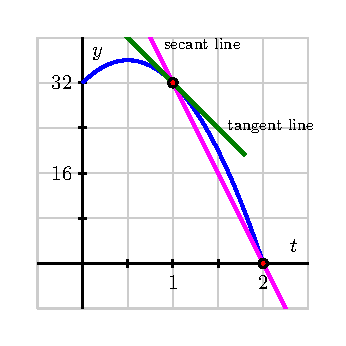
\includegraphics{figures/1_3_Act2Soln.eps}
	
	\item Observe that whenever the ball is rising, it's position function is rising, and thus the slope of its tangent line at any such point will be positive. This means that we should find $s'(a)$ to be positive whenever $0 \le a < \frac{1}{2}$, and similarly $s'(a)$ to be negative whenever $\frac{1}{2} < a < 2$ (which is when the ball is falling).  At the instant $a = \frac{1}{2}$, the ball is at its vertex and is neither rising nor falling, and at that point, $s'(\frac{1}{2}) = 0.$
\ea
\end{activitySolution}
\aftera % ACTIVITY  

\newpage

\begin{marginfigure}[1cm]
\margingraphics{figures/1_3_Act3.eps} 
\caption{Axes for plotting $y = P(t)$ in Activity~\ref{A:2.1.3}.} \label{fig:2.1.Act3}
\end{marginfigure}

\begin{activity}  \label{A:2.1.3}
A rapidly growing city in Arizona has its population $P$ at time $t$, where $t$ is the number of decades after the year $2010$, modeled by the formula $P(t) = 25000 e^{t/5}$.  Use this function to respond to the following questions.
\ba
	\item Sketch an accurate graph of $P$ for $t = 0$ to $t = 5$ on the axes provided in Figure~\ref{fig:2.1.Act3}.  Label the scale on the axes carefully.
	
	\item Compute the average rate of change of $P$ between $2030$ and $2050$.  Include units on your answer and write one sentence to explain the meaning (in everyday language) of the value you found.
	\item Use the limit definition to write an expression for the instantaneous rate of change of $P$ with respect to time, $t$, at the instant $a = 2$.  Explain why this limit is difficult to evaluate exactly.  
	\item Estimate the limit in (c) for the instantaneous rate of change of $P$ at the instant $a = 2$ by using several small $h$ values.  Once you have determined an accurate estimate of $P'(2)$, include units on your answer, and write one sentence (using everyday language) to explain the meaning of the value you found.
	\item On your graph above, sketch two lines:  one whose slope represents the average rate of change of $P$ on $[2,4]$, the other whose slope represents the instantaneous rate of change of $P$ at the instant $a=2$.
	\item In a carefully-worded sentence, describe the behavior of $P'(a)$ as $a$ increases in value.  What does this reflect about the behavior of the given function $P$?
\ea
\end{activity}
\begin{smallhint}
\ba
	\item $P(t)$ is the standard exponential function, scaled by $25000$.
	\item Use the formula for the average rate of change of a function.
	\item Because of the exponential nature of $P(t)$, we're not able to simplify $\frac{P(2+h)-P(2)}{h}$ in a way that removes $h$ from the denominator.  
	\item Try using $h = 0.001, 0.0001, 0.00001$ and $h = -0.001, -0.0001, -0.00001$.  Be careful not to round or use computing precision that is too limited.  
	\item For the first line, think about the points $(2,P(2))$ and $(4,P(4))$.
	\item Visualize the slope of the tangent line and how it changes as a point moves along the curve.
\ea
\end{smallhint}
\begin{bighint}
\ba
	\item $P(t)$ is the standard exponential function, scaled by $25000$.
	\item Remember that $AV_{[2,4]} = \frac{P(4)-P(2)}{4-2}$, and that the units on $P$ are people, while $t$ is the number of decades after 2010. 
	\item Note that
	$$P'(2) = \lim_{h \to 0} \frac{P(2+h)-P(2)}{h} = \lim_{h \to 0} \frac{25000 e^{2+h}-25000e^2}{h}.$$  
	\item Try using $h = 0.001, 0.0001, 0.00001$ and $h = -0.001, -0.0001, -0.00001$.  Be careful not to round or use computing precision that is too limited.  Think about how using the two values of $h$ nearest 0 together could give you the most accurate result.
	\item For the first line, think about the points $(2,P(2))$ and $(4,P(4))$.  For the second, try the line through $(2,P(2))$ with slope $P'(2)$.
	\item Visualize the slope of the tangent line and how it changes as a point moves along the curve.  Does the slope of the tangent line increase, decrease, or stay the same as the point of tangency moves along the curve from right to left?
\ea
\end{bighint}
\begin{activitySolution}
\ba
	\item 	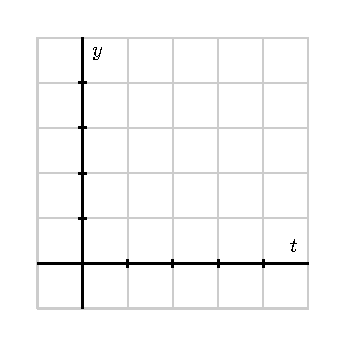
\includegraphics{figures/1_3_Act3.eps}
	\item $AV_{[2,4]} = \frac{P(4)-P(2)}{4-2} = \frac{25000e^{4/5} - 25000e^{2/5}}{2} \approx 9171$ people per decade is expected to be the average rate of change of the city's population over the two decades from 2030 to 2050.
	\item Note that
	\begin{eqnarray*} P'(2) & = & \lim_{h \to 0} \frac{P(2+h)-P(2)}{h} = \lim_{h \to 0} \frac{25000 e^{(2+h)/5}-25000e^{2/5}}{h} \\
	                                 & = &  \lim_{h \to 0} \frac{25000 e^{2/5} e^{h/5} -25000e^{2/5}}{h} =  \lim_{h \to 0} 25000e^{2/5}\left( \frac{e^{h/5} - 1}{h}\right)	\end{eqnarray*}
Because there is no way to remove a factor of $h$ from the numerator, we cannot eliminate the $h$ that is making the denominator go to zero, so it appears we need to be content estimating the limit with small values of $h$.
	\item Using $h = 0.00001$, we find $\frac{P(2+0.00001)-P(2)}{0.00001} \approx 7457$; using $h = -0.00001$, we find $\frac{P(2-0.00001)-P(2)}{-0.00001} \approx 7460$.  Averaging these two results, we find that
	$$P'(2) =  \lim_{h \to 0} \frac{P(2+h)-P(2)}{h} \approx 7458.5$$
	which is measured in people per decade.
	\item See the graph provided in (a) above.  The magenta line has slope equal to the average rate of change of $P$ on $[2,4]$, while the green line is the tangent line at $(2,P(2))$ with slope $P'(2)$.
	\item If we consider the point where $t = a$ and let $a$ start at 0 and then increase, it appears that the tangent line's slope at the point $(a,P(a))$ will increase as $a$ increases.
\ea
\end{activitySolution}
\aftera % ACTIVITY

%------------------------------------------------------------------
% SUBSECTION UNITS OF THE DERIVATIVE FUNCTION
%------------------------------------------------------------------
\subsection*{Units of the derivative function}

As we now know, the derivative of the function $f$ at a fixed value $x$ is given by
$$f'(x) = \ds \lim_{h \to 0} \frac{f(x+h)-f(x)}{h},$$  and this value has several different interpretations.  If we set $x = a$, one meaning of $f'(a)$ is  the slope of the tangent line at the point $(a,f(a))$.

In alternate notation, we also sometimes equivalently write $\frac{df}{dx}$ or $\frac{dy}{dx}$ instead of $f'(x)$, and these notations help us to further see the units (and thus the meaning) of the derivative as it is viewed as \emph{the instantaneous rate of change of $f$ with respect to $x$}\index{instantaneous rate of change}.  Note that the units on the slope of the secant line, $\frac{f(x+h)-f(x)}{h}$, are ``units of $f$ per unit of $x$.''  Thus, when we take the limit to get $f'(x)$, we get these same units on the derivative $f'(x)$:  units of $f$ per unit of $x$.  Regardless of the function $f$ under consideration (and regardless of the variables being used), it is helpful to remember that the units on the derivative function are ``units of output per unit of input,'' in terms of the input and output of the original function.

For example, say that we have a function $y = P(t)$, where $P$ measures the population of a city (in thousands) at the start of year $t$ (where $t = 0$ corresponds to $2010$ AD), and we are told that $P'(2) = 21.37$.  What is the meaning of this value?  Well, since $P$ is measured in thousands and $t$ is measured in years, we can say that the instantaneous rate of change of the city's population with respect to time at the start of $2012$ is $21.37$ thousand people per year.  We therefore expect that in the coming year, about $21,370$ people will be added to the city's population.

%----------------------------------------------------
% SUBSECTION ESTIMATING DERIVATIVES 
%----------------------------------------------------
\subsection*{Estimating Derivatives}

An interesting and powerful feature of mathematics is that it can often be thought of both in abstract terms and in applied ones.  For instance, calculus can be developed almost entirely as an abstract collection of ideas that focus on properties of arbitrary functions.  At the same time, calculus can also be very directly connected to our experience of physical reality by considering functions that represent meaningful processes.  We have already seen that for a position function $y = s(t)$, say for a ball being tossed straight up in the air, the ball's velocity at time $t$ is given by $v(t) = s'(t)$, the derivative of the position function.  Further, recall that if $s(t)$ is measured in feet at time $t$, the units on $v(t) = s'(t)$ are feet per second.

In what follows, we investigate several different functions, each with specific physical meaning, and think about how the units on the independent variable, dependent variable, and the derivative function add to our understanding.  To start, we consider the familiar problem of a position function of a moving object.

\begin{marginfigure}[8cm]
\margingraphics{figures/1_5_PA1.eps}
\caption{The graph of $y = s(t)$, the position of the car along highway $46$, which tells its distance in miles from Gackle, ND, at time $t$ in minutes.} \label{fig:2.1.Act4}
\end{marginfigure}

\begin{activity}  \label{A:2.1.4}
One of the longest stretches of straight (and flat) road in North America can be found on the Great Plains in the state of North Dakota on state highway $46$, which lies just south of the interstate highway I-$94$ and runs through the town of Gackle.  A car leaves town (at time $t = 0$) and heads east on highway $46$; its position in miles from Gackle at time $t$ in minutes is given by the graph of the function in Figure~\ref{fig:2.1.Act4}.  Three important points are labeled on the graph; where the curve looks linear, assume that it is indeed a straight line.

\ba
	\item In everyday language, describe the behavior of the car over the provided time interval.  In particular, discuss what is happening on the time intervals $[57,68]$ and $[68,104]$.
	\item Find the slope of the line between the points $(57,63.8)$ and $(104,106.8)$.  What are the units on this slope?  What does the slope represent?
	\item Find the average rate of change of the car's position on the interval $[68,104]$.  Include units on your answer.
	\item Estimate the instantaneous rate of change of the car's position at the moment $t = 80$.  Write a sentence to explain your reasoning and the meaning of this value.
\ea
\end{activity} % ACTIVITY

%-----------------------------------------------------------------------------------
% SUBSECTION TOWARD MORE ACCURATE DERIVATIVE ESTIMATES
%-----------------------------------------------------------------------------------
\subsection*{Toward more accurate derivative estimates}

It is also helpful to recall that when we want to estimate the value of $f'(x)$ at a given $x$, we can use the \emph{difference quotient} \index{difference quotient} $\frac{f(x+h)-f(x)}{h}$ with a relatively small value of $h$.  In doing so, we should use both positive and negative values of $h$ in order to make sure we account for the behavior of the function on both sides of the point of interest.  To that end, we consider the following brief example to demonstrate the notion of a \emph{central difference} and its role in estimating derivatives.

\begin{example} \label{Ex:2.1.Eg2}
Suppose that $y = f(x)$ is a function for which three values are known:  $f(1) = 2.5$, $f(2) = 3.25$, and $f(3) = 3.625$.  Estimate $f'(2)$.

\solution We know that $\ds f'(2) = \lim_{h \to 0} \frac{f(2+h) - f(2)}{h}$.  But since we don't have a graph for $y = f(x)$ nor a formula for the function, we can neither sketch a tangent line nor evaluate the limit exactly.  We can't even use smaller and smaller values of $h$ to estimate the limit.  Instead, we have just two choices:  using $h = -1$ or $h = 1$, depending on which point we pair with $(2,3.25)$.

So, one estimate is
$$f'(2) \approx \frac{f(1)-f(2)}{1-2} = \frac{2.5-3.25}{-1} = 0.75.$$
The other is
$$f'(2) \approx \frac{f(3)-f(2)}{3-2} = \frac{3.625-3.25}{1} = 0.375.$$
Since the first approximation looks only backward from the point $(2,3.25)$ and the second approximation looks only forward from $(2,3.25)$, it makes sense to average these two values in order to account for behavior on both sides of the point of interest.  Doing so, we find that
$$f'(2) \approx \frac{0.75 + 0.375}{2} = 0.5625.$$
\end{example} % EXAMPLE

\begin{marginfigure}[1cm] % MARGIN FIGURE
\margingraphics{figures/1_5_Ex1.eps}
\caption{At left, the graph of $y = f(x)$ along with the secant line through $(1,2.5)$ and $(2,3.25)$, the secant line through $(2, 3.25)$ and $(3,3.625)$, as well as the tangent line.  At right, the same graph along with the secant line through $(1,2.5)$ and $(3,3.625)$, plus the tangent line.}\label{fig:2.1.Eg2}
\end{marginfigure}

The intuitive approach to average the two estimates found in Example~\ref{Ex:2.1.Eg2} is in fact the best possible estimate to $f'(2)$ when we have just two function values for $f$ on opposite sides of the point of interest.  To see why, we think about the diagram in Figure~\ref{fig:2.1.Eg2}, which shows a possible function $y = f(x)$ that satisfies the data given in Example~\ref{Ex:2.1.Eg2}.  On the left, we see the two secant lines with slopes that come from computing the \emph{backward difference} \index{backward difference} $\frac{f(1)-f(2)}{1-2} = 0.75$ and from the \emph{forward difference} \index{forward difference} $\frac{f(3)-f(2)}{3-2} = 0.375.$  Note how the first such line's slope over-estimates the slope of the tangent line at $(2,f(2))$, while the second line's slope underestimates $f'(2)$.  On the right, however, we see the secant line whose slope is given by the \emph{central difference} \index{central difference} 
\[ \frac{f(3)-f(1)}{3-1} = \frac{3.625-2.5}{2} = \frac{1.125}{2} = 0.5625.\]

Note that this central difference has the exact same value as the average of the forward difference and backward difference (and it is straightforward to explain why this always holds), and moreover that the central difference yields a very good approximation to the derivative's value, in part because the secant line that uses both a point before and after the point of tangency yields a line that is closer to being parallel to the tangent line.  

In general, the central difference approximation to the value of the first derivative is given by 
$$f'(a) \approx \frac{f(a+h) - f(a-h)}{2h},$$
and this quantity measures the slope of the secant line to $y = f(x)$ through the points $(a-h, f(a-h))$ and $(a+h, f(a+h))$. Anytime we have symmetric data surrounding a point at which we desire to estimate the derivative, the central difference is an ideal choice for so doing.

The following activities will further explore the meaning of the derivative in several different contexts while also viewing the derivative from graphical, numerical, and algebraic perspectives.

\begin{margintable}[8cm]
\begin{center}
\scalebox{1.5}{
\begin{tabular}{| l || l |}
\hline
$t$ & $F(t)$ \\ \hline \hline
$0$ & $70$\\ \hline
$15$ & $180.5$ \\ \hline
$30$ & $251$ \\ \hline
$45$ & $296$ \\ \hline
$60$ & $324.5$ \\ \hline
$75$ & $342.8$ \\ \hline
$90$ & $354.5$  \\ \hline
\end{tabular}
} % end scalebox 
\caption{The temperature of a potato in an oven at various times.} \label{T:2.1.5}
\end{center}
\end{margintable}

\begin{activity} \label{A:2.1.5}
A potato is placed in an oven, and the potato's temperature $F$ (in degrees Fahrenheit) at various points in time is taken and recorded in Table~\ref{T:2.1.5}. Time $t$ is measured in minutes.

\ba
	\item Use a central difference to estimate the instantaneous rate of change of the temperature of the potato at $t= 30$. Include units on your answer. 
	\item Use a central difference to estimate the instantaneous rate of change of the temperature of the potato at $t= 60$. Include units on your answer. 
	\item Without doing any calculation, which do you expect to be greater: $F'(75)$ or $F'(90)$?  Why?
	\item Suppose it is given that $F(64) = 330.28$ and $F'(64) = 1.341$.  What are the units on these two quantities?  What do you expect the temperature of the potato to be when $t = 65$?  when $t = 66$?  Why?
	\item Write a couple of careful sentences that describe the behavior of the temperature of the potato on the time interval $[0,90]$, as well as the behavior of the instantaneous rate of change of the temperature of the potato on the same time interval.
\ea

\end{activity}
\begin{smallhint}
\ba
	\item Think about quantities such as $\frac{F(45)-F(30)}{45-30}$.
	\item See the note in (a).
	\item Is $F$ changing faster at $t = 75$ or at $t = 90$?
	\item Remember that the units on $F'$ will be ``degrees Fahrenheit per minute.''
	\item Be careful to distinguish between the temperature, $F$, and the rate of change of temperature, $F'$, in your commentary.
\ea
\end{smallhint}
\begin{bighint}
\ba
	\item Think about quantities such as $\frac{F(45)-F(30)}{45-30}$ and $\frac{F(15)-F(30)}{15-30}$.
	\item See the note in (a).
	\item What overall trend do you observe in the instantaneous rate of change of $F$, based on the overall trend in temperature $F$?
	\item Remember that the units on $F'$ will be ``degrees Fahrenheit per minute.''
	\item Be careful to distinguish between the temperature, $F$, and the rate of change of temperature, $F'$, in your commentary.
\ea
\end{bighint}
\begin{activitySolution}
\ba
	\item Using the central difference, we find that 
	$$F'(30) \approx \frac{F(45)-F(15)}{45-15} = \frac{296-180.5}{30} = 3.85$$
	degrees per minute.
	\item Using the central difference, we find that 
	$$F'(60) \approx \frac{F(75)-F(45)}{45-15} = \frac{342.8-296}{30} = 1.56$$
	degrees per minute.
	\item Over each subsequent time interval, we see that the amount of increase in the potato's temperature gets less and less, thus we expect the value of $F'(t)$ to get smaller and smaller as time goes on.  We therefore expect $F'(75) > F'(90)$.
	\item The value $F(64) = 330.28$ is the temperature of the potato in degrees Fahrenheit at time 64, while $F'(64) = 1.341$ measures the instantaneous rate of change of the potato's temperature with respect to time at the instant $t = 64$, and its units are degrees per minute.  Because at time $t = 64$ the potato's temperature is increasing at 1.341 degrees per minute, we expect that at $t = 65$, the temperature will be about 1.341 degrees greater than at $t = 64$, or in other words $F(65) \approx 330.28 + 1.341 = 331.621$.  Similarly, at $t = 66$, two minutes have elapsed from $t = 64$, so we expect an increase of $2 \dot 1.341$ degrees:  $F(66) \approx 330.28 + 2 \cdot 1.341 = 332.962$. 
	\item Throughout the time interval $[0,90]$, the temperature $F$ of the potato is increasing.  But as time goes on, the rate at which the temperature is rising appears to be decreasing.  That is, while the values of $F$ continue to get larger as time progresses, the values of $F'$ are getting smaller (while still remaining positive). We thus might say that ``the temperature of the potato is increasing, but at a decreasing rate.''
\ea
\end{activitySolution}
\aftera %ACTIVITY

\begin{example} \label{Ex:2.1.Eg4}
A company manufactures rope, and the total cost of producing $r$ feet of rope is $C(r)$ dollars.  What does it mean to say that $C(2000) = 800$? What are the units of $C'(r)$? Suppose that $C(2000) = 800$ and $C'(2000) = 0.35$.  Estimate $C(2100)$, and justify your estimate by writing at least one sentence that explains your thinking. Which of the following statements do you think is true, and why?
	\begin{itemize}
		\item $C'(2000) < C'(3000)$
		\item $C'(2000) = C'(3000)$
		\item $C'(2000) > C'(3000)$
	\end{itemize}
Suppose someone claims that $C'(5000) = -0.1$.  What would the practical meaning of this derivative value tell you about the approximate cost of the next foot of rope?  Is this possible?  Why or why not?  
	
\solution When we say $C(2000) = 800$, we mean that the total cost of producing $2000$ feet of rope is $800$ dollars.  Remember that the units on any derivative are ``units of output per unit of input,'' and the units of $C'(r)$ are ``dollars per foot.''

If $C(2000) = 800$ and $C'(2000) = 0.35$, then we know once $2000$ feet of rope are produced, the total cost function is increasing at $\$0.35$ per additional foot of rope.  Then, if we manufacture an additional $100$ feet of rope, the additional total cost will be approximately 
\[ 100 \ \mbox{feet} \cdot 0.35 \ \frac{\mbox{dollars}}{\mbox{foot}} = 35 \ \mbox{dollars}. \]
Therefore, we find that $C(2100) \approx C(2000) + 35 = 835,$ or that the cost to make $2100$ feet of rope is about $\$835$.

Either $C'(2000) = C'(3000)$ or $C'(2000) > C'(3000)$, since we expect the cost per foot of additional rope to either stay constant or to get smaller as the production volume increases.  Said differently, the instantaneous rate of change of the total cost function should either be constant or decrease due to economy of scale.

It is impossible to have $C'(5000) = -0.1$ and indeed to have any negative derivative value for the total cost function.  The total cost function $C(r)$ can never decrease, because it doesn't make sense for the total cost of producing $5001$ feet of rope to be less than the total cost of producing $5000$ feet of rope.

\end{example} %ACTIVITY  %this is a lot of activities we may need to narrow

\begin{activity} \label{A:2.1.7}
Researchers at a major car company have found a function that relates gasoline consumption to speed for a particular model of car.  In particular, they have determined that the consumption $C$, in {\bfseries liters per kilometer}, at a given speed $s$, is given by a function $C = f(s)$, where $s$ is the car's speed in {\bf kilometers per hour}. 
	\ba
	  \item Data provided by the car company tells us that $f(80) = 0.015$, $f(90) = 0.02$, and $f(100) = 0.027$.  Use this information to estimate the instantaneous rate of change of fuel consumption with respect to speed at $s = 90$.  Be as accurate as possible, use proper notation, and include units on your answer.
	  \item By writing a complete sentence, interpret the meaning (in the context of fuel consumption) of ``$f(80) = 0.015$.'' 
	  \item Write at least one complete sentence that interprets the meaning of the value of $f'(90)$ that you estimated in (a).
	\ea
\end{activity}
\begin{smallhint}
\ba
	\item Try a central difference.
	\item What is happening when the car is traveling at 80 km/hr?
	\item Remember that units on the derivative are ``units of output per unit of input.''
\ea
\end{smallhint}
\begin{bighint}
\ba
	\item Remember that $f'(a) \approx \frac{f(a+h)-f(a-h)}{2h}$ and use appropriate values of $a$ and $h$.
	\item Complete the following sentence: ``When the car is traveling at 80 kilometers per hour, it is using fuel at a rate of 0.015 $\ldots$''
	\item Remember that units on the derivative are ``units of output per unit of input,'' even when the input and/or output are rates themselves.
\ea
\end{bighint}
\begin{activitySolution}
\ba
	\item Using a central difference, we have
	$$f'(90) = \frac{f(100) - f(80}{100-80} = \frac{0.027 - 0.015}{20} = \frac{0.012}{20} = 0.0006$$
	which tells us that $f'(90) = 0.0006$ liters per kilometer per kilometer per hour.
	\item When the car is traveling at 80 kilometers per hour, it is using fuel at a rate of 0.015 liters per kilometer.  That is, at the given speed, for each additional kilometer the car travels, it uses an additional 0.015 liters of fuel.
	\item To say that $f'(90) = 0.0006$ liters per kilometer per kilometer per hour means that when the car is traveling at 90 kilometers per hour, its rate of fuel consumption per kilometer is increasing at a rate of 0.0006 liters per kilometer per kilometer per hour.  If we increase our speed from 90 to 91 km/hr, we would expect our rate of fuel consumption to rise by 0.0006 liters for each additional kilometer driven.
\ea
\end{activitySolution}
\aftera %ACTIVITY

%--------------
% SUMMARY
%--------------
\begin{summary}
\item The average rate of change of a function $f$ on the interval $[a,b]$ is $\ds \frac{f(b)-f(a)}{b-a}$.  The units on the average rate of change are units of $f$ per unit of $x$, and the numerical value of the average rate of change represents the slope of the secant line between the points $(a,f(a))$ and $(b,f(b))$ on the graph of $y = f(x)$.  If we view the interval as being $[a,a+h]$ instead of $[a,b]$, the meaning is still the same, but the average rate of change is now computed by  $\ds \frac{f(a+h)-f(a)}{h}$.

\item The instantaneous rate of change with respect to $x$ of a function $f$ at a value $x = a$ is denoted $f'(a)$ (read ``the derivative of $f$ evaluated at $a$'' or ``$f$-prime at $a$'') and is defined by the formula
$$f'(a) = \lim_{h \to 0} \frac{f(a+h)-f(a)}{h},$$
provided the limit exists.  Note particularly that the instantaneous rate of change at $x = a$ is the limit of the average rate of change on $[a,a+h]$ as $h \to 0$.

\item Provided the derivative $f'(a)$  exists, its value tells us the instantaneous rate of change of $f$ with respect to $x$ at $x = a$, which geometrically is the slope of the tangent line to the curve $y = f(x)$ at the point $(a,f(a))$.  We even say that $f'(a)$ is the \emph{slope of the curve} $y = f(x)$ at the point $(a,f(a))$.

\item Limits are the link between average rate of change and instantaneous rate of change: they allow us to move from the rate of change over an interval to the rate of change at a single point.

%\item Regardless of the context of a given function $y=f(x)$, the derivative always measures the instantaneous rate of change of the output variable with respect to the input variable.

%\item The units on the derivative function $y = f'(x)$ are units of $f$ per unit of $x$.  Again, this measures how fast the output of the function $f$ changes when the input of the function changes.

\item The central difference approximation to the value of the first derivative is given by 
$$f'(a) \approx \frac{f(a+h) - f(a-h)}{2h},$$
and this quantity measures the slope of the secant line to $y = f(x)$ through the points $(a-h, f(a-h))$ and $(a+h, f(a+h))$.  The central difference generates a good approximation of the derivative's value any time we have symmetric data surrounding a point of interest.

\item Knowing the derivative and function values at a single point enables us to estimate other function values nearby.  If, for example, we know that $f'(7) = 2$, then we know that at $x = 7$, the function $f$ is increasing at an instantaneous rate of $2$ units of output for every one unit of input.  Thus, we expect $f(8)$ to be approximately $2$ units greater than $f(7)$.  The value is approximate because we don't know that the rate of change stays the same as $x$ changes.
\end{summary}

\clearpage

%--------------
% EXERCISES
%--------------
\begin{adjustwidth*}{}{-2.25in}
\textbf{{\large Exercises}}
\setlength{\columnsep}{25pt}
\begin{multicols*}{2}
\noindent Terms and Concepts \small
\begin{enumerate}[1)]
\item {T/F: Let $f$ be a position function. The average rate of change on $[a,b]$ is the slope of the line through the points $(a, f(a))$ and $(b,f(b))$.}
\item {T/F: The definition of the derivative of a function at a point involves taking a limit.}
\item {In your own words, explain the difference between the average rate of change and instantaneous rate of change.}
\item What is the instantaneous rate of change of position called?
\item Given a function $y=f(x)$, in your own words describe how to find the units of $f'(x)$.
\item Let $V(x)$ measure the volume, in decibels, measured inside a restaurant with $x$ customers. What are the units of $V'(x)$?
\item Let $v(t)$ measure the velocity, in ft/s, of a car moving in a straight line $t$ seconds after starting. What are the units of $v'(t)$?
\end{enumerate} 

\noindent {\normalsize Problems} \small

\noindent {\bf In exercises 8--14, a function and an $x$-value $a$ are given.
\begin{enumerate}[a),leftmargin=12pt]
\item Find the derivative of the function at the given point.
\item Find the tangent line to the graph of the function at $a$.
\end{enumerate}}

\begin{enumerate}[1),resume]
\item $\ds f(x) = 6; \quad a = -2$
\item $\ds f(x) = 2x; \quad a = 3$
\item $\ds h(x) = 4 - 3x; \quad a = 7$
\item $\ds g(x) = x^2; \quad a = 2$
\item $\ds f(x) = 3x^2 - x + 4; \quad a = -1$
\item $\ds h(x) = \frac{1}{x}; \quad a = -2$
\item $\ds r(x) = \frac{1}{x-2}; \quad a = 3$
\end{enumerate}

\noindent {\bf In exercises 15--17, use a central difference to estimate the instantaneous rates of change at the indicated values.}
\begin{enumerate}[1),resume]
\item The yearly profits $P(t)$, in millions of dollars, of a certain company from $1990$ to $1996$ are given in the following table.

\scalebox{0.85}{\begin{tabular}{|c|c|c|c|c|c|c|c|}
\hline
Year & $1990$ & $1991$ & $1992$ & $1993$ & $1994$ & $1995$ & $1996$ \\ \hline
Profit & $0.5$ & $1.0$ & $1.2$ & $1.6$ & $2.5$ & $1.6$ & $2.0$ \\ \hline
\end{tabular}}% end scalebox

Estimate $P'(1991)$, $P'(1993)$, and $P'(1995)$.  Include units in your answers.

\item The position, $s(t)$, of an object moving in a straight line at time $t$ is given by the following table.

\begin{center}
\scalebox{0.85}{\begin{tabular}{|c|c|c|c|c|c|}
\hline
$t$ & $0$ & $0.5$ & $1$ & $1.5$ & $2$  \\ \hline
$s(t)$ & $0$ & $30$ & $52$ & $66$ & $72$  \\ \hline
\end{tabular}}% end scalebox
\end{center}

Estimate $s'(0.5)$, $s'(1)$, and $s'(1.5)$.  Include units in your answers.

\item The average price, $p(t)$, for a ticket to a movie theater in North America for selected years is shown in the following table.

 \scalebox{0.85}{\begin{tabular}{|c|c|c|c|c|c|c|c|}
\hline
Year & $1987$ & $1991$ & $1995$ & $1999$ & $2003$ & $2007$ & $2009$ \\ \hline
Price (\$) & $3.91$ & $4.21$ & $4.35$ & $5.06$ & $6.03$ & $6.88$ & $7.50$ \\ \hline
\end{tabular}}% end scalebox

{\footnotesize (Source: National Association of Theater Owners, www.natoonline.org)}

\ba
\item Estimate $p'(1991)$ and $p'(2003)$.  Include units in your answers.
\item Are we able to estimate $p'(2007)$ using a central difference?  Why or why not?
\ea

\item A cup of coffee has its temperature $F$ (in degrees Fahrenheit) at time $t$ given by the function $F(t) = 75 + 110 e^{-0.05t}$, where time is measured in minutes.
\ba
\item Use a central difference with $h = 0.01$ to estimate the value of $F'(10)$.
\item What are the units on the value of $F'(10)$ that you computed in (a)?  What is the practical meaning of the value of $F'(10)$?
\item Which do you expect to be greater: $F'(10)$ or $F'(20)$?  Why?  
\item Write a sentence that describes the behavior of the function $y = F'(t)$ on the time interval $0 \le t \le 30$.  How do you think its graph will look?  Why?
\ea

\item The temperature change $T$ (in Fahrenheit degrees), in a patient, that is generated by a dose $q$ (in milliliters), of a drug, is given by the function $T = f(q)$.
\ba
\item What does it mean to say $f(50) = 0.75$?  Write a complete sentence to explain, using correct units.
\item A person's sensitivity, $s$, to the drug is defined by the function $s(q) = f'(q)$.  What are the units of sensitivity?
\item Suppose that $f'(50) = -0.02$.  Write a complete sentence to explain the meaning of this value.  Include in your response the information given in (a).
\ea

\end{enumerate}

%------------------------------------------
% END OF EXERCISES ON FIRST PAGE
%------------------------------------------
\end{multicols*}
\end{adjustwidth*}

\clearpage

\begin{adjustwidth*}{}{-2.25in}
\setlength{\columnsep}{25pt}
\begin{multicols*}{2}\small

\begin{enumerate}[1),start=20]
\item The velocity of a ball that has been tossed vertically in the air is given by $v(t) = 16 - 32t$, where $v$ is measured in feet per second, and $t$ is measured in seconds.  The ball is in the air from $t = 0$ until $t = 2$.
\ba
\item When is the ball's velocity greatest?
\item Determine the value of $v'(1)$.  Justify your thinking.
\item What are the units on the value of $v'(1)$?  What does this value and the corresponding units tell you about the behavior of the ball at time $t = 1$?  
\item What is the physical meaning of the function $v'(t)$?
\ea

\item The value, $V$, of a particular automobile (in dollars) depends on the number of miles, $m$, the car has been driven, according to the function $V = h(m)$.  
\ba
\item Suppose that $h(40000) = 15500$ and $h(55000) = 13200$.  What is the average rate of change of $h$ on the interval $[40000,55000]$, and what are the units on this value?
\item In addition to the information given in (a), say that $h(70000) = 11100$.  Determine the best possible estimate of $h'(55000)$ and write one sentence to explain the meaning of your result, including units on your answer.
\item Which value do you expect to be greater: $h'(30000)$ or $h'(80000)$?  Why?
\item Write a sentence to describe the long-term behavior of the function $V = h(m)$, plus another sentence to describe the long-term behavior of $h'(m)$.  Provide your discussion in practical terms regarding the value of the car and the rate at which that value is changing.
\ea

\end{enumerate}

%------------------------------------------------
% END OF EXERCISES ON SECOND PAGE
%------------------------------------------------
\end{multicols*}
\end{adjustwidth*}
\afterexercises 

\cleardoublepage